\documentclass{article}

\usepackage[a4paper, top=2cm, bottom=2cm, left=2cm, right=2cm]{geometry}
\usepackage[utf8]{vietnam}
\usepackage{amsmath, nccmath}
\usepackage{setspace}
\usepackage{scrextend}
\usepackage{adjustbox}
\usepackage{graphicx}
\usepackage{icomma}
\usepackage{siunitx}
\usepackage{fancyhdr}

\pagestyle{fancy}
\fancyhf{}
\rhead{Nguyễn Minh Đăng - 20230022}
\fancyfoot[C]{\thepage}
\changefontsizes{13pt}

\begin{document}
\onehalfspacing
{
   \setlength{\topmargin}{-0.5cm}
\begin{titlepage}
  \begin{center}
    \centerline{
\includegraphics[height=42mm]{logo}}

    
   \vspace{1cm}

        {\large Trường Đại học Khoa học Tự nhiên}\\[1em]
        {\large Đại học Quốc gia Thành phố Hồ Chí Minh}
    
        \vspace{1.2cm}
    \centerline{\hbox to 13cm{\hrulefill}}
    \vspace{0.3cm}
    \Large  {{Thực Tập Chuyên Đề 1 }}
    \centerline{\hbox to 13cm{\hrulefill}}
    
    \vspace{1.2cm}
    \Large {Bài 8: Suy Giảm Của Chùm Tia Gamma Qua Vật Chất}\\ 
   
   \vspace{3cm}
            \large Người hướng dẫn: Thầy Lê Hoàng Minh \\ 
            \large Sinh viên: Nguyễn Minh Đăng - 20230022
    
    \vspace{4cm}
    

    
    \hbox to \textwidth{\hrulefill}
    \vspace{0.2cm}
    {\sc  11/04/2023}
    
  \end{center}
\end{titlepage}
}

\newpage
\clearpage\thispagestyle{empty}\addtocounter{page}{-1} 
\clearpage
\mbox{}
 % creates a blank space to fill the page
\newpage
\section*{\centering Báo Cáo Thực Nghiệm}
\vspace{1cm}

\setcounter{section}{1}

\subsection{Phương trình hồi quy}
Ta có công thức suy giảm qua vật liệu
\begin{align*}
	I_d = I_0e^{-\mu d}
\end{align*}
Do $I_0$ là một dữ liệu đo được từ máy thí nghiệm, nên nó không thể hoàn toàn giống với lý thuyết. Thế ta sẽ đặt $I_0$ là một nghiệm ẩn và tìm phương trình hồi quy. \\
Ta có:
\begin{align*}
	& ln(I_d) = ln(I_0) - \mu d \\
	& v_i = ln(I_0) - \mu d - ln(I_d) \\
	& S = \sum_{i=1}^{n}v_i^2 =\sum_{i=1}^{n}\Big[ ln(I_0) - \mu d - ln(I_d) \Big]^2 \\
	& S = \sum_{i=1}^{n}\Big[ln^2(I_0) + \mu^2d^2 + ln^2(I_d) - 2ln(I_0)ln(I_d) - 2ln(I_0)\mu d + 2\mu dln(I_d) \Big]
\end{align*}
Để tìm được thông số $a_r$ thì ta đặt cho $S$ là cực tiểu:
\begin{align*}
	\rightarrow \frac{\partial S}{\partial a_r} = 0
\end{align*}
Từ đây ta có:
\begin{itemize} 
	\item $\begin{aligned}
				 \frac{\partial S}{\partial \mu} = 2\mu d^2 - 2ln(I_0)d + 2dln(I_d) = 0
\end{aligned}$
\end{itemize}
\begin{align}
	\rightarrow \mu \sum{d^2} - ln(I_0)\sum{d} = - \sum{dln(I_d)}
\end{align}
\begin{itemize} 
	\item $\begin{aligned}
				 \frac{\partial S}{\partial ln(I_0)} = 2ln(I_0) - 2ln(I_d) - 2\mu d = 0
\end{aligned}$
\end{itemize}
\begin{align}
	\rightarrow -\mu \sum{d} + nln(I_0) =  \sum{ln(I_d)}
\end{align}
Từ (1) và (2) ta có hệ phương trình
\begin{align}
	\begin{cases}
	\mu \sum{d^2} - ln(I_0)\sum{d} = - \sum{dln(I_d)} \\ 
	-\mu \sum{d} + nln(I_0) =  \sum{ln(I_d)} 
	\end{cases}
\end{align}
\vspace{0.5cm}

\subsection{Sai số lan truyền}
Từ các dữ liệu thực nghiệm ta có được phương trình
\begin{align*}
	I_d = \frac{I_0}{t}e^{-\mu d} - \frac{G}{t}
\end{align*}
Với: \begin{fleqn}[\parindent]
\begin{equation*}
\begin{split}
	&t: \text{Thời gian đo} \\ 
	&d: \text{Bề dày vật liệu} \\
	&I_d: \text{Tốc độ đếm trung bình qua vật liệu} \\
	&I_0: \text{Tốc độ đếm trung bình khi chưa qua vật liệu} \\
	&G: \text{Tốc độ đếm phông trung bình}
\end{split}
\end{equation*}
\end{fleqn}
Ta chỉ tính sai số của $I_d$ và $G$ vì $d$ không có dữ liệu
\begin{itemize} 
	\item $\begin{aligned}
				 \frac{\partial I_d}{\partial I_0} = \frac{e^{-\mu d}}{t}
\end{aligned}$
	\item $\begin{aligned}
				 \frac{\partial I_d}{\partial G} = -\frac{1}{t}
\end{aligned}$
\end{itemize}
Từ đây ta có
\begin{align*}
	\sigma_{Id} = \sqrt{ \frac{I_0e^{-2\mu d}}{t^2} + \frac{G}{t^2} }
\end{align*}
Từ đây ta thấy sai số sẽ thay đổi tùy theo bề dày vậy liệu
\vspace{0.5cm}

\subsection{Vật liệu Cu}
Nguồn: Co-60, hoạt độ: 1 $\mu Ci$ \\
Thời gian đo: 60 s
\begin{table}[!ht]
    \centering
    \begin{adjustbox}{max width=\textwidth}
    \begin{tabular}{|c|c|c|c|c|c|c|c|c|c|}
    \hline
        Bề dày d (mm) & 0 & 1,01 & 2,02 & 3,02 & 4,02 & Số đếm phông (số đếm/s)  \\ \hline
        Số đếm tổng (số đếm/s) & 1,35 & 1,15 & 1,08 & 1,06 & 1,02 & 0,40   \\ \hline
        Sai số số đếm thực (số đếm/s) & 0,17 & 0,16 & 0,15 & 0,15 & 0,14 &  \\ \hline
        Số đếm thực (số đếm/s) & 0,95 & 0,76 & 0,68 & 0,67 & 0,62 &  \\ \hline
    \end{tabular}
    \end{adjustbox}
\end{table} \\
Từ đây ta có các số
\begin{align*}
	& \sum{d^2} = 30,38; \ \quad \sum{d} = 10,07 \\
	& \sum{d.ln(I_d)} = -4,19; \ \quad \sum{ln(I_d)} = -1,59
\end{align*}
Từ đây ta có hệ phương trình
\begin{align*}
	\begin{cases}
	30,38\mu - 10.07ln(I_0) = - (-4,19) \\ 
	-10,07\mu + 5ln(I_0) =  -1,59
	\end{cases}
	\rightarrow
	\begin{cases}
	\mu = 0,10 \ (mm^{-1}) \\
	ln(I_0) = -0,12 \rightarrow I_0 = 0,89 \ \text{(số đếm/s)}
	\end{cases}
\end{align*}
Ta có hệ số suy giảm khối
\begin{align*}
	\mu_m = \frac{\mu}{\rho_{Cu}} = \frac{0,01}{8,96} = 1,\num{12e-2} \ (g/cm^3)
\end{align*}
Ta có bề dày một nữa
\begin{align*}
	\Delta_{1/2} = \frac{1}{\mu}ln(2) = \frac{1}{0,1}ln(2) = 6,93 \ (mm)
\end{align*}
Từ đây ta có phương trình hồi quy
\begin{align*}
	I_d = 0,89e^{-0,10d}
\end{align*}
Ta có đồ thị
\begin{center}
  {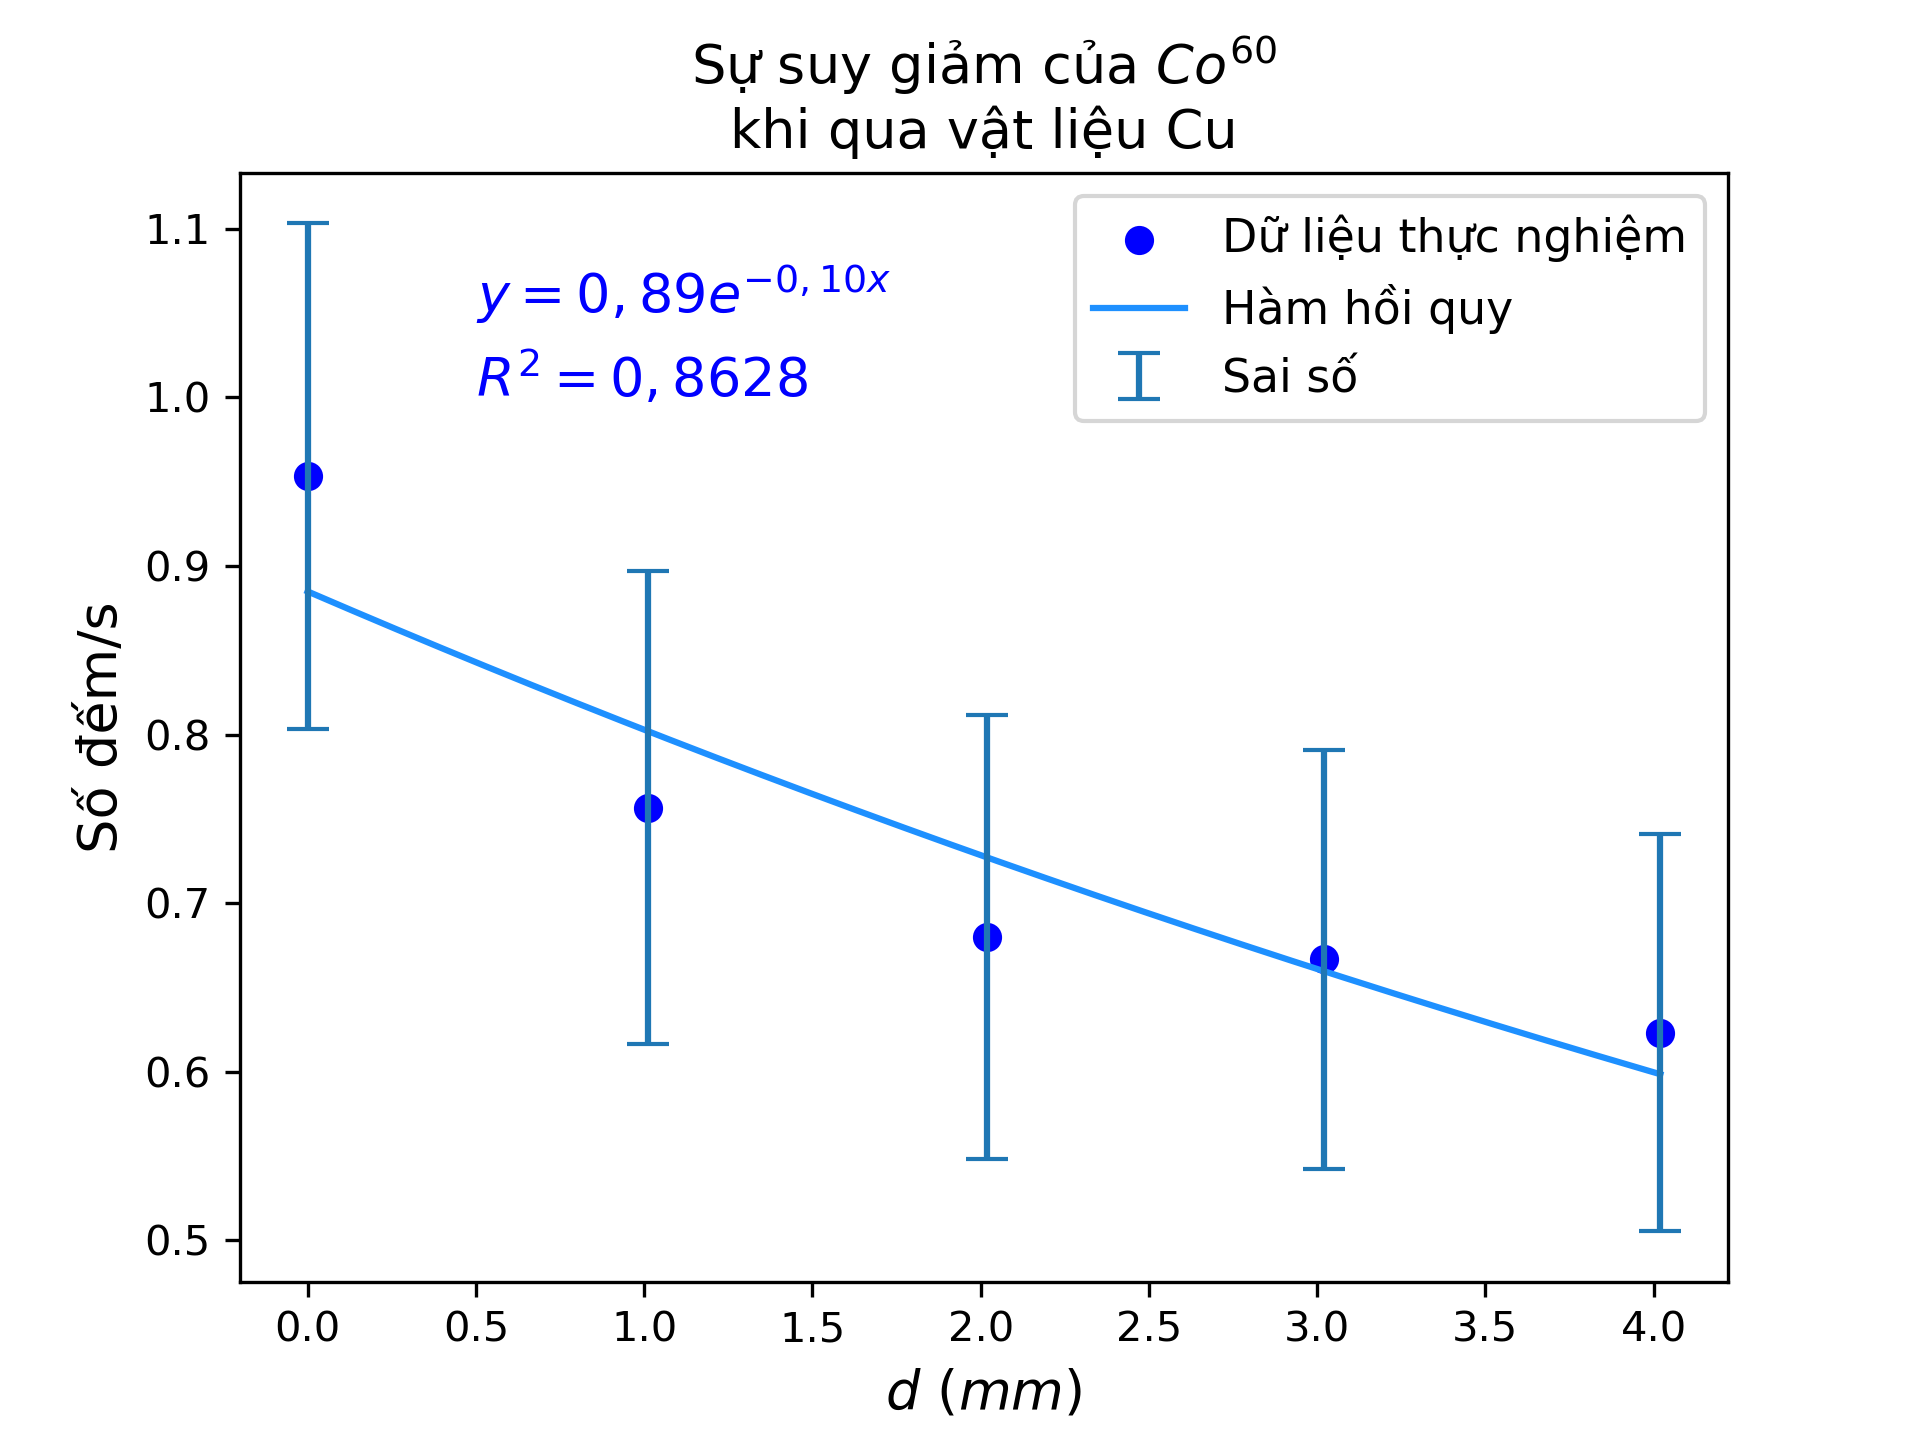
\includegraphics[width=\textwidth]{cu}}
\end{center}
\vspace{0.5cm}

\newpage
\subsection{Vật liệu Al}
Nguồn: Cs-137, hoạt độ: 400 $kBq$ \\
Thời gian đo: 5 phút \\
Máy đo số đếm chứ không phải tốc độ đếm
\begin{table}[!ht]
    \centering
    \begin{tabular}{|c|c|c|c|c|c|c|}
    \hline
        Bề dày d (mm) & 0 & 20,07 & 45,75 & 70,75  \\ \hline
        Số đếm tổng (số đếm) & 12729 & 8594 & 4972 & 2966  \\ \hline
        Sai số số đếm thực (số đếm) & 112,82 & 92,70 & 70,51 & 54,46  \\ \hline
    \end{tabular}
\end{table}\\
Từ đây ta có các số
\begin{align*}
	& \sum{d^2} = 7501,43; \ \quad \sum{d} = 136,57 \\
	& \sum{d.ln(I_d)} = 1136,86; \ \quad \sum{ln(I_d)} = 35,02
\end{align*}
Từ đây ta có hệ phương trình
\begin{align*}
	\begin{cases}
	7501,43\mu - 136,57ln(I_0) = - 1136,86 \\ 
	-136,57\mu + 4ln(I_0) =  35,02
	\end{cases}
	\rightarrow
	\begin{cases}
	\mu = 0,02 \ (mm^{-1}) \\
	ln(I_0) = 9,46 \rightarrow I_0 = 12835,88 \ \text{(số đếm)}
	\end{cases}
\end{align*}
Ta có hệ số suy giảm khối
\begin{align*}
	\mu_m = \frac{\mu}{\rho_{Al}} = \frac{0,002}{2,7} = 7,\num{41e-4} \ (g/cm^3)
\end{align*}
Ta có bề dày một nữa
\begin{align*}
	\Delta_{1/2} = \frac{1}{\mu}ln(2) = \frac{1}{0,02}ln(2) = 34,66 \ (mm)
\end{align*}
Từ đây ta có phương trình hồi quy
\begin{align*}
	I_d = 12835,88e^{-0,02d}
\end{align*}
\newpage
Từ đây ta có đồ thị
\begin{center}
  {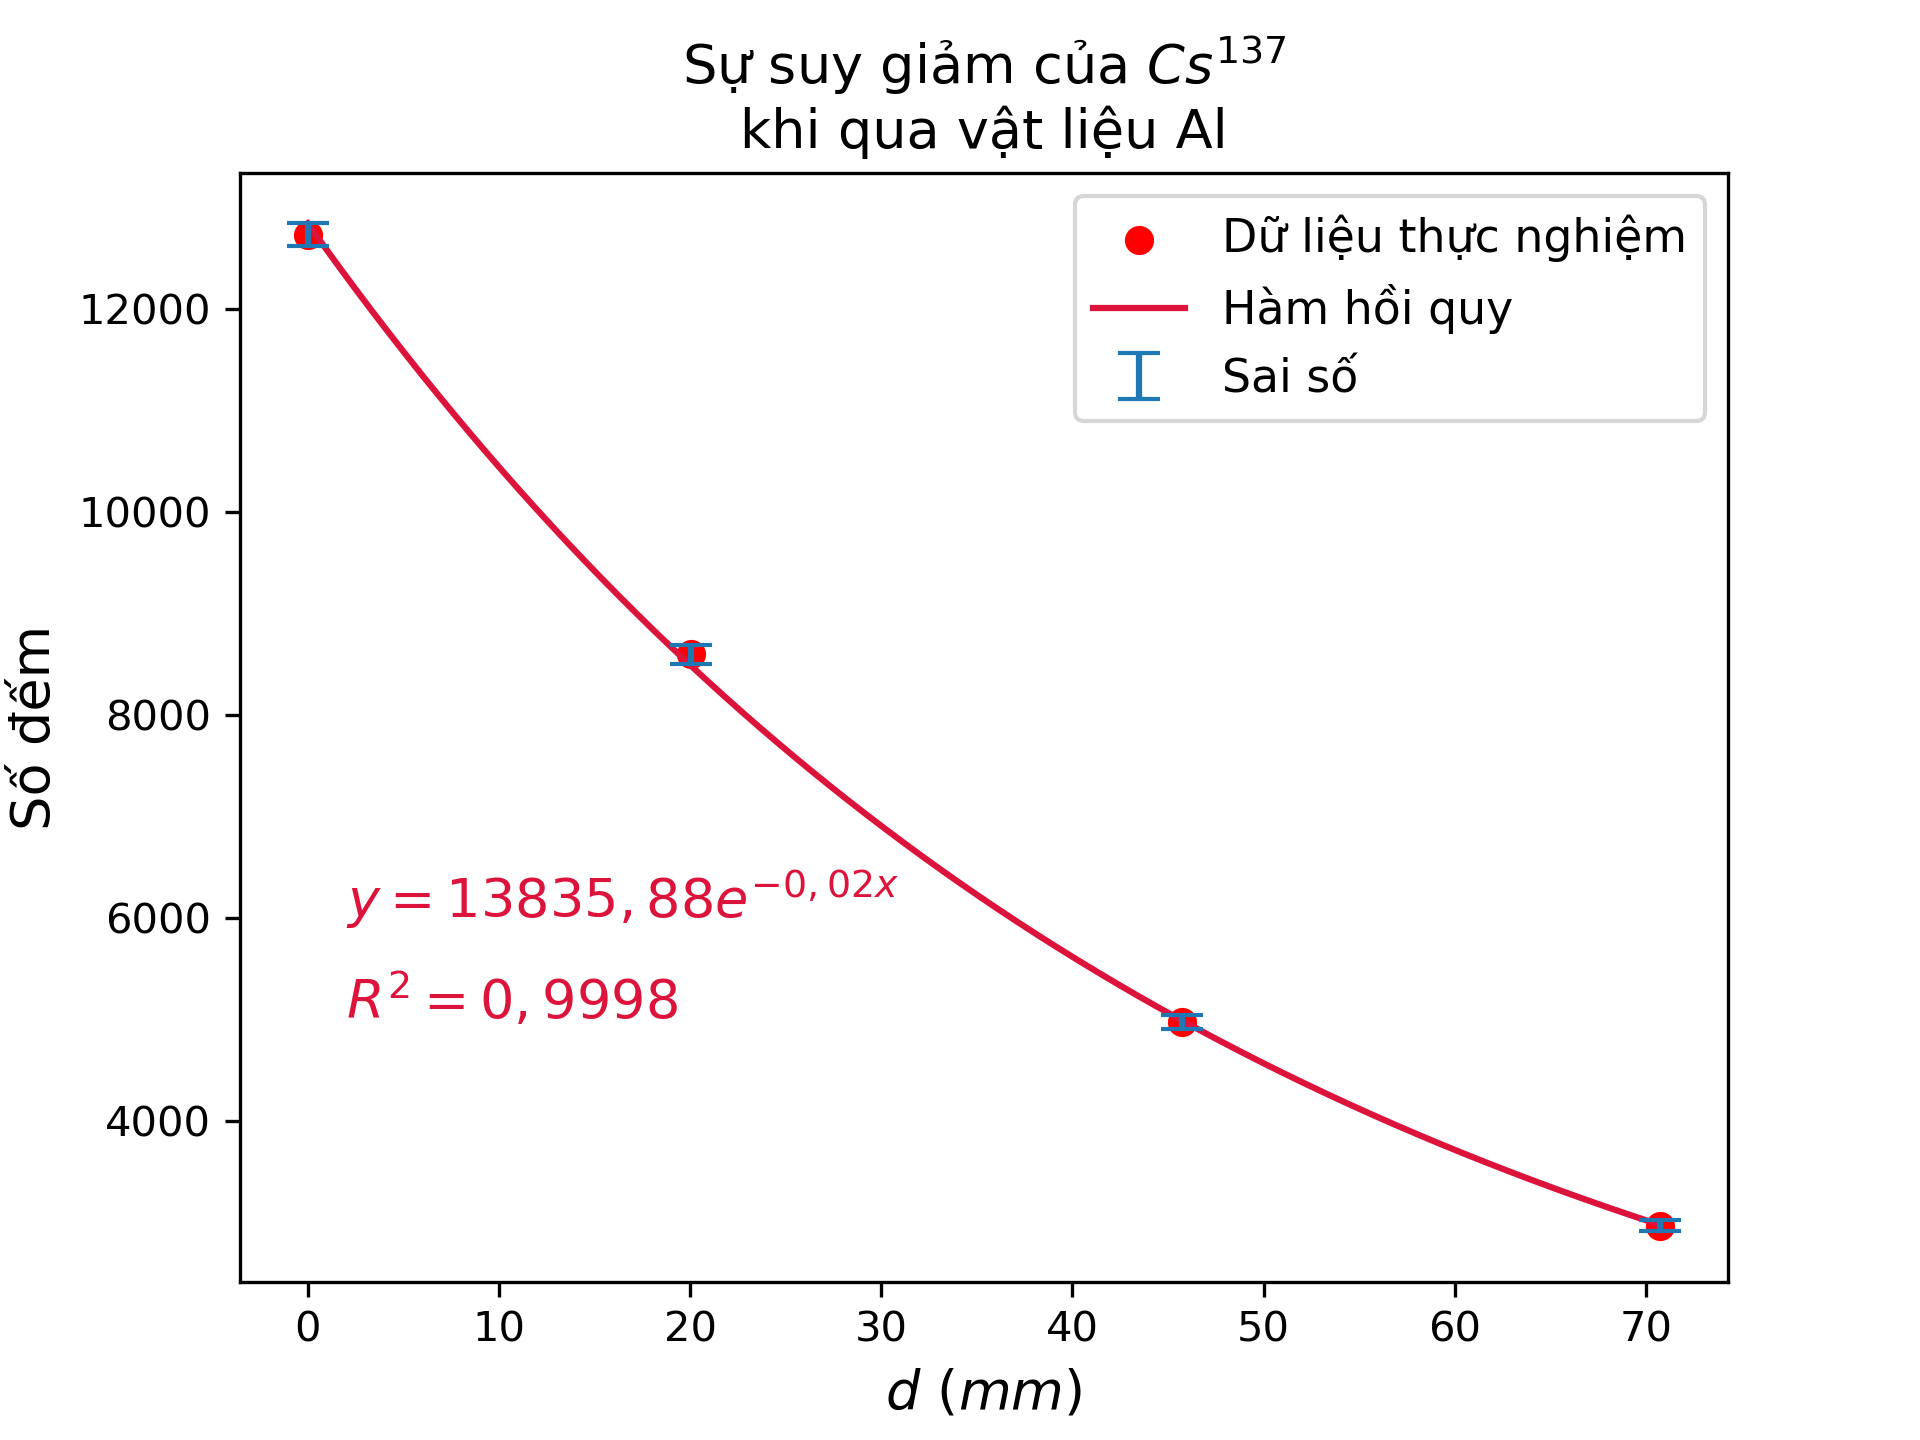
\includegraphics[width=\textwidth]{al}}
\end{center}
\vspace{0.5cm}

\subsection{Vật liệu Pb}
Nguồn: Ra-226, hoạt độ: 9 $\mu Ci$ \\
Thời gian đo: 5 phút \\
\begin{table}[!ht]
    \centering
    \begin{tabular}{|c|c|c|c|c|c|c|}
    \hline
        Bề dày d (mm) & 0 & 3.05 & 10.47 & 16.58 & Số đếm phông (số đếm/s)  \\ \hline
        Số đếm tổng (số đếm/s) & 30.35 & 1.23 & 0.95 & 0.74 & 0.31   \\ \hline
        Sai số số đếm thực (số đếm/s) & 0.32 & 0.19 & 0.06 & 0.04 &  \\ \hline
        Số đếm thực (số đếm/s) & 30.04 & 0.91 & 0.64 & 0.43  & \\ \hline
    \end{tabular}
\end{table}\\
Từ đây ta có các số
\begin{align*}
	& \sum{d^2} = 393,82; \ \quad \sum{d} = 30,10 \\
	& \sum{d.ln(I_d)} = -18,95; \ \quad \sum{ln(I_d)} = 2,02
\end{align*}
Từ đây ta có hệ phương trình
\begin{align*}
	\begin{cases}
	393,82\mu - 30,10ln(I_0) = - (-18,95) \\ 
	-30,10\mu + 4ln(I_0) =  2,02
	\end{cases}
	\rightarrow
	\begin{cases}
	\mu = 0,20\ (mm^{-1}) \\
	ln(I_0) = 2,04 \rightarrow I_0 = 7,69 \ \text{(số đếm/s)}
	\end{cases}
\end{align*}
Ta có hệ số suy giảm khối
\begin{align*}
	\mu_m = \frac{\mu}{\rho_{Pb}} = \frac{0,02}{11,3} = 1,\num{77e-3} \ (g/cm^3)
\end{align*}
Ta có bề dày một nữa
\begin{align*}
	\Delta_{1/2} = \frac{1}{\mu}ln(2) = \frac{1}{0,2}ln(2) = 3,47 \ (mm)
\end{align*}
Từ đây ta có phương trình hồi quy
\begin{align*}
	I_d = 7,69e^{-0,2d}
\end{align*}
Từ đây ta có đồ thị
\begin{center}
  {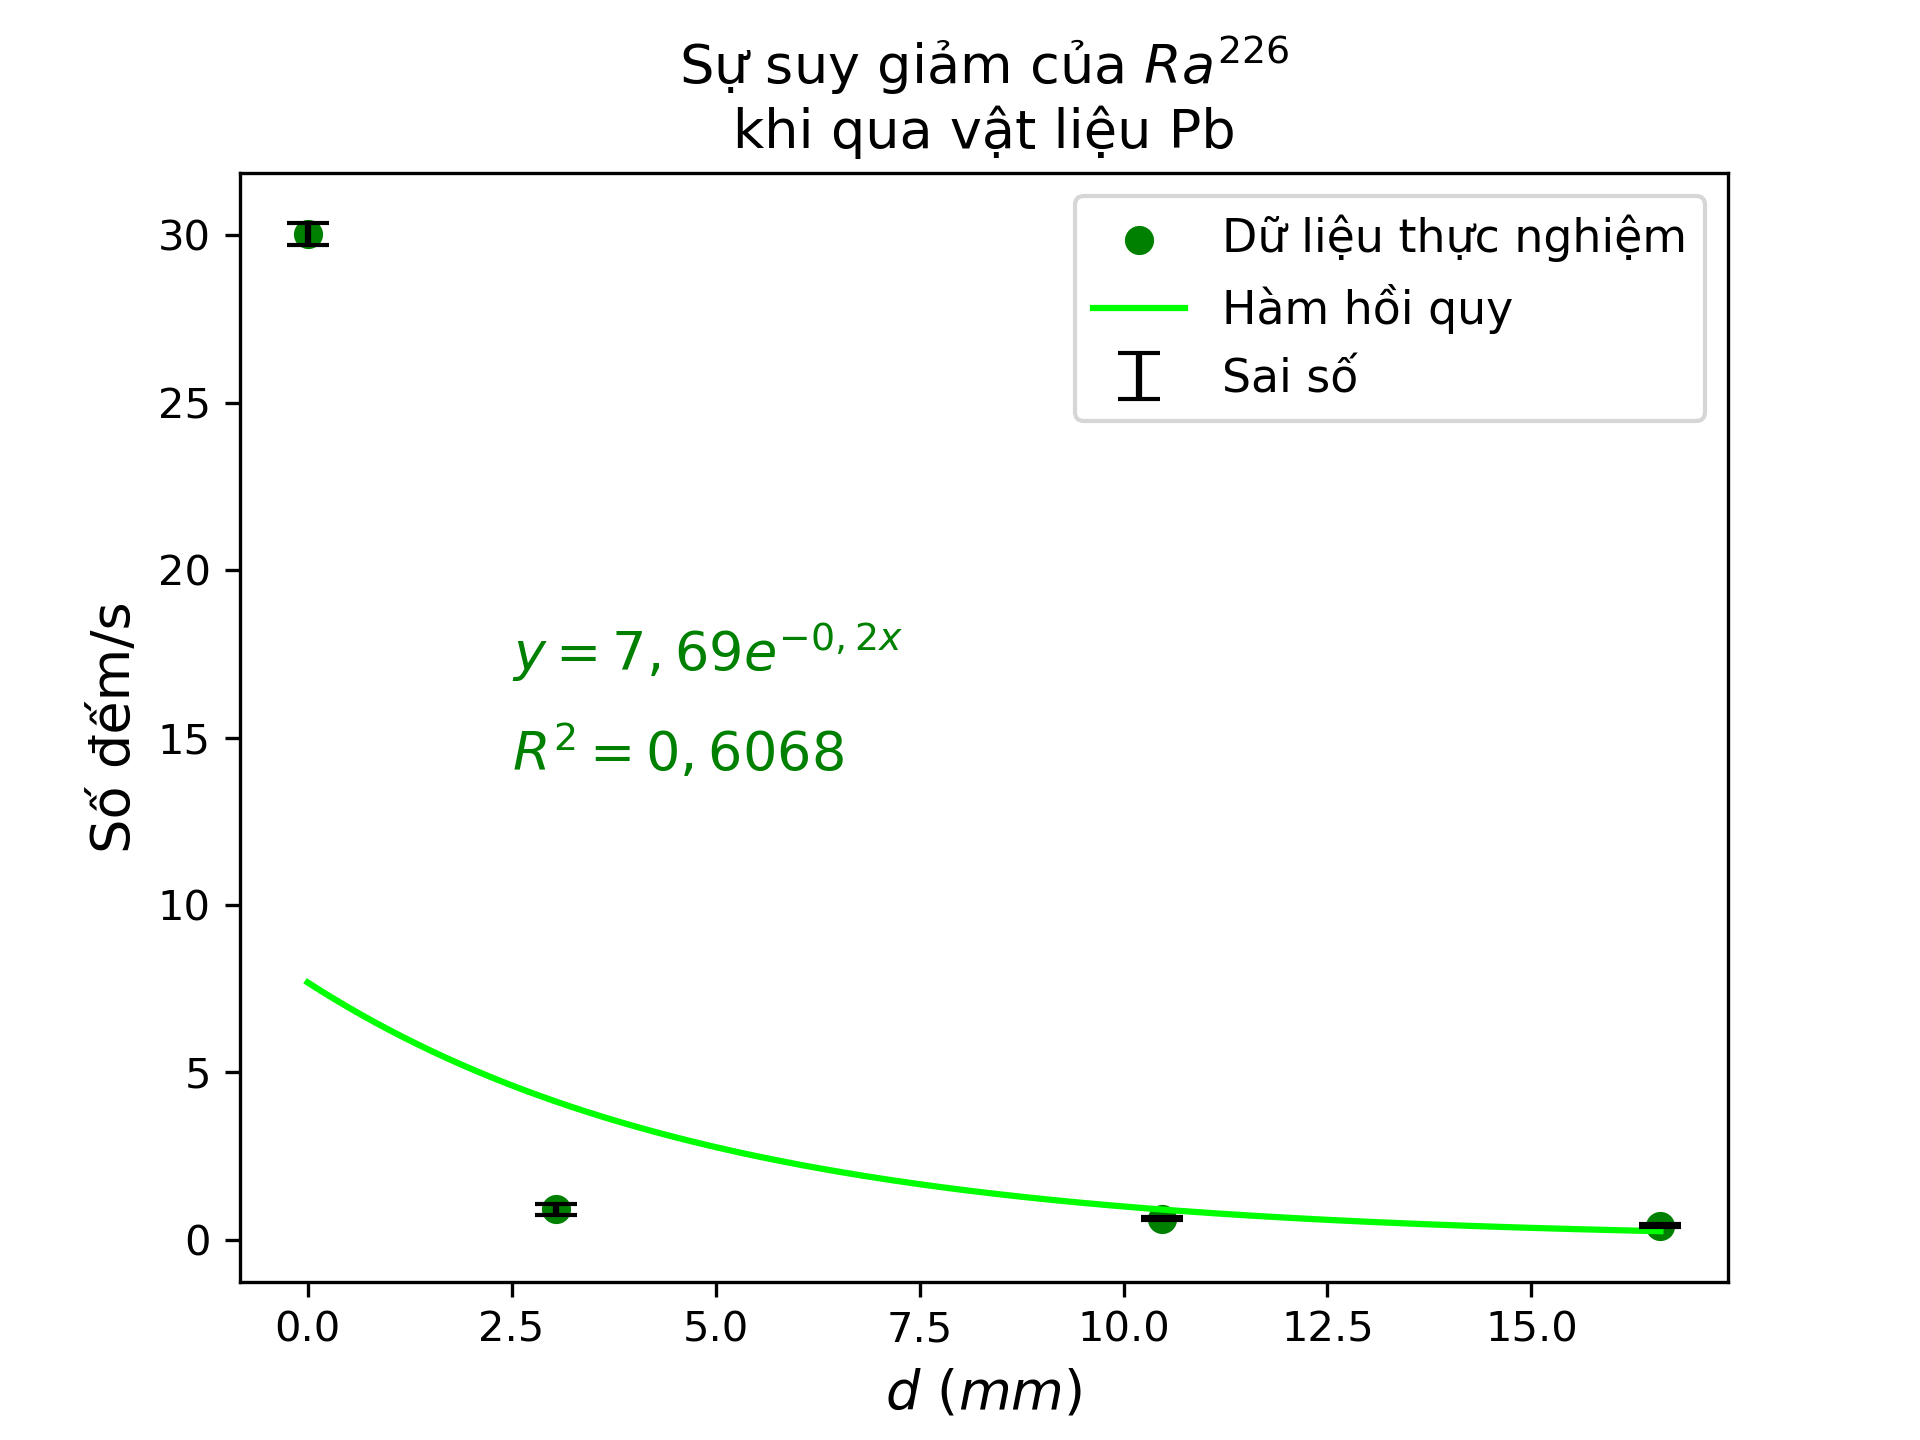
\includegraphics[width=\textwidth]{pb}}
\end{center}

\newpage
\clearpage\thispagestyle{empty}\addtocounter{page}{-1} 
\clearpage
\mbox{}
 % creates a blank space to fill the page
\newpage


\end{document}